\let\negmedspace\undefined
\let\negthickspace\undefined
\documentclass[journal]{IEEEtran}
\usepackage[a5paper, margin=10mm, onecolumn]{geometry}
%\usepackage{lmodern} % Ensure lmodern is loaded for pdflatex
\usepackage{tfrupee} % Include tfrupee package

\setlength{\headheight}{1cm} % Set the height of the header box
\setlength{\headsep}{0mm}     % Set the distance between the header box and the top of the text

\usepackage{gvv-book}
\usepackage{gvv}
\usepackage{cite}
\usepackage{amsmath,amssymb,amsfonts,amsthm}
\usepackage{algorithmic}
\usepackage{graphicx}
\usepackage{textcomp}
\usepackage{xcolor}
\usepackage{txfonts}
\usepackage{listings}
\usepackage{enumitem}
\usepackage{mathtools}
\usepackage{gensymb}
\usepackage{comment}
\usepackage[breaklinks=true]{hyperref}
\usepackage{tkz-euclide} 
\usepackage{listings}
% \usepackage{gvv}                                        
\def\inputGnumericTable{}                                 
\usepackage[latin1]{inputenc}                                
\usepackage{color}                                            
\usepackage{array}                                            
\usepackage{longtable}                                       
\usepackage{calc}                                             
\usepackage{multirow}                                         
\usepackage{hhline}                                           
\usepackage{ifthen}                                           
\usepackage{lscape}
\usepackage{circuitikz}
\tikzstyle{block} = [rectangle, draw, fill=blue!20, 
    text width=4em, text centered, rounded corners, minimum height=3em]
\tikzstyle{sum} = [draw, fill=blue!10, circle, minimum size=1cm, node distance=1.5cm]
\tikzstyle{input} = [coordinate]
\tikzstyle{output} = [coordinate]

\begin{document}

\bibliographystyle{IEEEtran}
\vspace{3cm}

\title{4.13.100}
\author{AI25BTECH110031 \\ Shivam Sawarkar}
 \maketitle
% \newpage
% \bigskip
{\let\newpage\relax\maketitle}

\renewcommand{\thefigure}{\theenumi}
\renewcommand{\thetable}{\theenumi}
\setlength{\intextsep}{10pt} % Space between text and floats


\numberwithin{equation}{section}
\numberwithin{figure}{enumi}
\renewcommand{\thetable}{\theenumi}

\textbf{Question(4.13.100)} Let $\vec{S}$ be the reflection of a point $\vec{Q}$ with respect to the plane given by $\vec{r}=-(t+p)\hat{i}+t\hat{j}+(1+p)\hat{k}$ where $t$, $p$ are real parameters and $\hat{i}$, $\hat{j}$, $\hat{k}$ are the unit vectors along the three positive coordinate axes. If the position vectors of $\vec{Q}$ and $\vec{S}$ are $10\hat{i}+15\hat{j}+20\hat{k}$ and $\alpha\hat{i}+\beta\hat{j}+\gamma\hat{k}$ respectively, then which of the following is/are TRUE ? \\ 
\begin{enumerate}[label=\alph*]
    \item $3(\alpha+\beta) = -101$
    \item $3(\beta+\gamma) = -71$
    \item $3(\gamma+\alpha) = -86$
    \item $3(\alpha+\beta+\gamma) = -121$
\end{enumerate}
\textbf{Solution:}

The plane is given by 
\begin{align}
\vec{r} = t\myvec{-1 \\ 1 \\ 0}+p\myvec{-1 \\ 0 \\ 1}+\myvec{0 \\ 0 \\ 1}
\end{align} 
so two direction vectors are
\begin{align}
\vec{u} = \myvec{-1\\1\\0}, 
\qquad 
\vec{v} = \myvec{-1\\0\\1}.
\end{align}

Hence the normal vector is
\begin{align}
\vec{n} = \vec{u} \times \vec{v} 
= \myvec{1\\1\\1}.
\end{align}

So the plane equation becomes
\begin{align}
\vec{n}^\top\vec x = 1.
\end{align}

For a point $\vec q \in \mathbb{R}^3$, its reflection across the plane 
$\vec{n}^\top\vec{x} = 1$ is
\begin{align}
\vec{S} = \vec{Q}-2\frac{\vec{n}^\top\vec{Q}-1}{\norm{n}^2}\vec{n},
\end{align}

Here
\begin{align}
\vec{n} = \myvec{1\\1\\1},  
\quad \vec{Q} = \myvec{10\\15\\20}.
\end{align}

\begin{align}
\vec{n}^\top\vec n = 1^2+1^2+1^2=3.
\end{align}


\begin{align}
\vec{S}=\myvec{\alpha \\ \beta \\ \gamma} = \myvec{\frac{58}{3} \\ -\frac{43}{3} \\ -\frac{28}{3}}.
\end{align}

\begin{align}
3(\alpha+\beta) = -101,\quad
3(\beta+\gamma) = -71,\quad
3(\gamma+\alpha) = -86,\quad
3(\alpha+\beta+\gamma) = -129.
\end{align}

Hence, the correct options are
\begin{align}
\boxed{(a), (b), (c)}.
\end{align}

\begin{figure}[H]
    \centering
    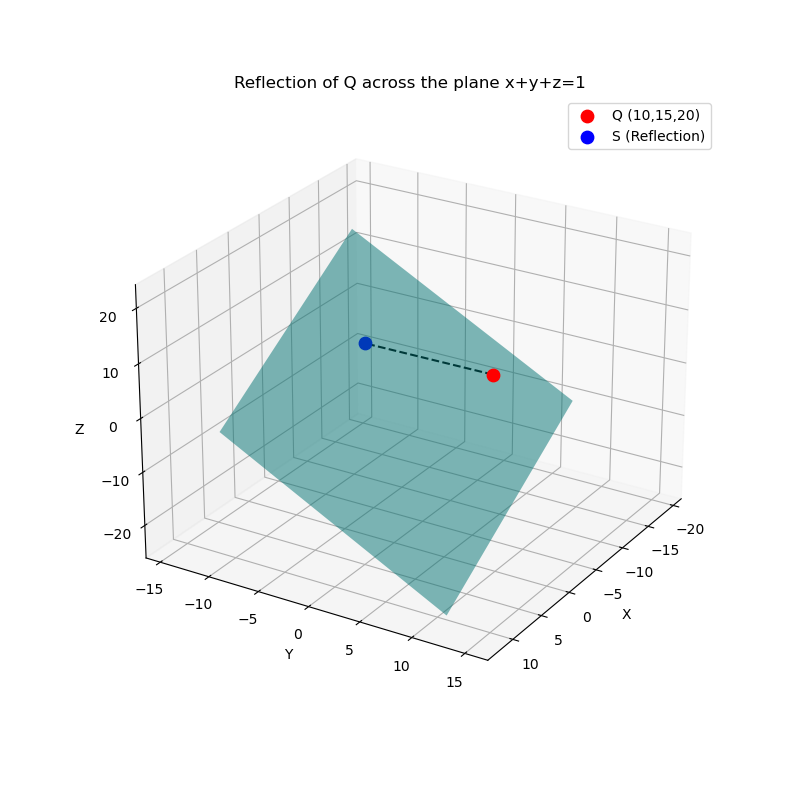
\includegraphics[width=0.8\linewidth]{figs/plot10.png}
    \caption{}
    \label{fig:placeholder}
\end{figure}




\end{document}